\chapter{Diseño del sistema}\label{diseno-del-sistema}

Este capítulo presenta el diseño del sistema desarrollado: la sección~\ref{arquitectura-general} describe la arquitectura en capas, la sección~\ref{arquitectura-del-array-tiledb} el esquema del array TileDB, la sección~\ref{proceso-de-carga-etl-geotiff_to_tiledb_sparse.py} el proceso de ingesta, la sección~\ref{gestion-de-multiples-escenarios-argumento---dataset} la gestión de múltiples escenarios y la sección~\ref{benchmark-de-almacenamiento} la elección experimental de la configuración de almacenamiento.

\section{Arquitectura general}\label{arquitectura-general}

El sistema está compuesto por cuatro capas articuladas en torno al array TileDB sparse como componente central de almacenamiento, tal y como muestra la Figura~\ref{fig:arquitectura}:

\begin{enumerate}
\item \textbf{Ingesta (ETL):} El módulo de ingesta lee los ficheros GeoTIFF generados por Triton, aplica el filtro de celdas húmedas (H $\geq$ 0,01 m) y escribe los datos en TileDB con filtro ByteShuffle+ZSTD-9. La lectura se realiza por franjas de 5\,000 filas para limitar el uso de memoria.
\item \textbf{Almacenamiento:} Array TileDB sparse con dimensiones (time, row, col) y atributos (H, QX, QY, MH). Un fragmento por paso temporal facilita el filtrado temporal eficiente.
\item \textbf{Análisis:} El motor de consultas proporciona 24 funciones que operan directamente sobre el array TileDB sin exportación previa.
\item \textbf{Visualización y exportación:} Un visualizador interactivo, un exportador a GeoTIFF para interoperabilidad SIG y la aplicación web Streamlit con mapas interactivos, comparativa multi-escenario y panel de ayuda.
\end{enumerate}

\begin{figure}[ht]
\centering
\begin{tikzpicture}[
    font=\small\sffamily,
    node distance=10mm,
    source/.style={rectangle, draw=black!70, fill=black!5, minimum height=11mm, minimum width=22mm, align=center, rounded corners=2pt},
    process/.style={rectangle, draw=blue!70!black, fill=blue!10, minimum height=11mm, minimum width=22mm, align=center, rounded corners=2pt, thick},
    storage/.style={cylinder, draw=orange!80!black, fill=orange!15, shape border rotate=90, aspect=0.25, minimum height=14mm, minimum width=26mm, align=center, thick},
    consumer/.style={rectangle, draw=green!50!black, fill=green!10, minimum height=10mm, minimum width=24mm, align=center, rounded corners=2pt},
    ui/.style={rectangle, draw=red!70!black, fill=red!8, minimum height=10mm, minimum width=28mm, align=center, rounded corners=2pt, thick},
    arrow/.style={-Latex, thick, draw=black!60},
]
    \node[source] (geo) {GeoTIFF Triton\\\scriptsize 1 escenario de simulación};
    \node[process, right=14mm of geo] (etl) {ETL\\\scriptsize filtrado y compresión};
    \node[storage, right=14mm of etl] (tdb) {TileDB sparse\\\scriptsize solo celdas húmedas};

    \node[consumer, below=14mm of tdb, xshift=-32mm] (queries) {Motor de consultas\\\scriptsize 24 funciones analíticas};
    \node[consumer, below=14mm of tdb, xshift=4mm] (viz) {Visualizador};
    \node[consumer, below=14mm of tdb, xshift=40mm] (exp) {Exportador GeoTIFF};

    \node[ui, below=12mm of viz] (app) {Aplicación web Streamlit};

    \draw[arrow] (geo) -- (etl);
    \draw[arrow] (etl) -- (tdb);
    \draw[arrow] (tdb.south) -- ++(0,-3mm) -| (queries.north);
    \draw[arrow] (tdb.south) -- ++(0,-3mm) -| (viz.north);
    \draw[arrow] (tdb.south) -- ++(0,-3mm) -| (exp.north);
    \draw[arrow] (queries.south) -- (app.north);
\end{tikzpicture}
\caption{Arquitectura del sistema en cuatro capas en torno al array TileDB sparse.}
\label{fig:arquitectura}
\end{figure}

\section{Arquitectura del array TileDB}\label{arquitectura-del-array-tiledb}

El array disperso se define con tres dimensiones y cuatro atributos, tal y como se muestra en la Tabla~\ref{tab:array-schema}. Las dimensiones (\texttt{time}, \texttt{row}, \texttt{col}) indexan cada celda húmeda dentro del cubo espacio-temporal, y los cuatro atributos almacenan los valores físicos de esa celda, de modo que una sola consulta puede recuperar cualquier combinación de variables sobre cualquier rango de tiempo y espacio.

\begin{table}[ht]
\centering
\begin{tabularx}{\textwidth}{>{\raggedright\arraybackslash}p{3cm}>{\raggedright\arraybackslash}p{2cm}L}
\toprule
\textbf{Elemento} & \textbf{Tipo} & \textbf{Detalles} \\
\midrule
Dimensión time & int32 & Índice del paso temporal (0--19) \\
Dimensión row & int32 & Fila del ráster (0--34\,199) \\
Dimensión col & int32 & Columna del ráster (0--23\,039) \\
\addlinespace[4pt]
Atributo H & float32 & Profundidad instantánea \\
Atributo QX & float32 & Caudal unitario X \\
Atributo QY & float32 & Caudal unitario Y \\
Atributo MH & float32 & Profundidad máxima histórica \\
\bottomrule
\end{tabularx}
\caption{Dimensiones y atributos del array TileDB sparse.}
\label{tab:array-schema}
\end{table}

La Figura~\ref{fig:tiledb-estructura} ilustra cómo TileDB organiza físicamente estos datos \cite{tiledb_indexing, tiledb_datalayout}: 20 fragmentos independientes (uno por paso temporal) almacenan únicamente las coordenadas y valores de las celdas húmedas, con los cuatro atributos codificados juntos mediante ByteShuffle+ZSTD-9. Cada celda húmeda guarda sus tres coordenadas enteras y los cuatro valores float32; las celdas secas ($\sim$92 \% del dominio) no se almacenan, y esta combinación es la que reduce los $\sim$235 GB originales a $\sim$17,5 GB.

\begin{figure}[ht]
\centering
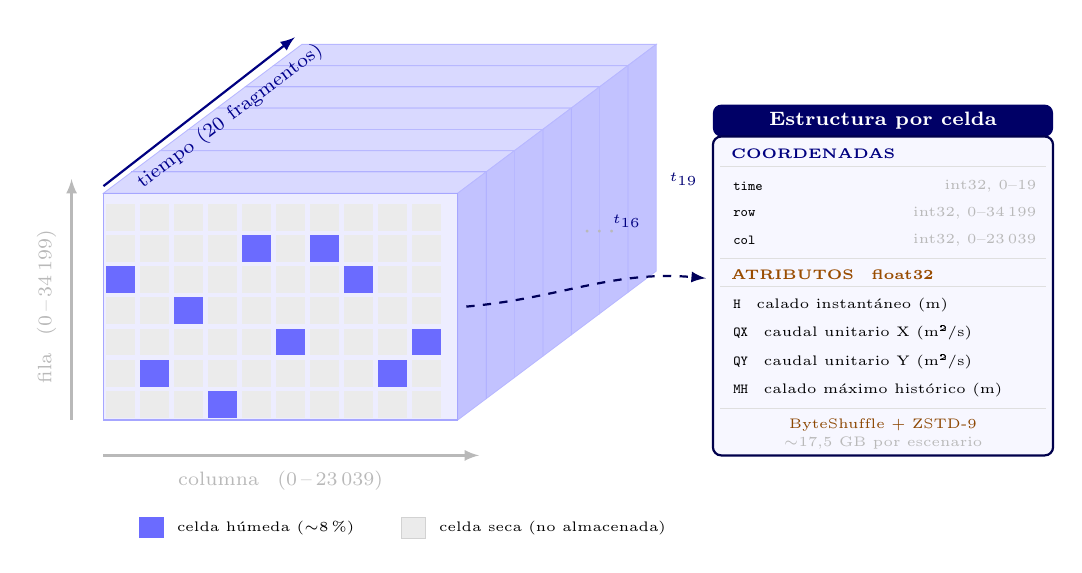
\begin{tikzpicture}[x=0.9cm, y=0.9cm, font=\small\sffamily]

  %% ── Parámetros (evitar \cs y \rs que son palabras reservadas TeX)
  \pgfmathsetmacro{\FW}{5.0}    % ancho cara frontal
  \pgfmathsetmacro{\FH}{3.2}    % alto cara frontal
  \pgfmathsetmacro{\OX}{0.40}   % offset oblicuo X
  \pgfmathsetmacro{\OY}{0.30}   % offset oblicuo Y
  \pgfmathsetmacro{\CW}{0.48}   % ancho celda mini-grid
  \pgfmathsetmacro{\CH}{0.44}   % alto celda mini-grid

  %% ── Stack de 7 fragmentos (de atrás a delante) ──────────────────
  \foreach \k in {6,5,4,3,2,1,0} {
    \pgfmathsetmacro{\DX}{\k*\OX}
    \pgfmathsetmacro{\DY}{\k*\OY}
    % Cara superior
    \fill[blue!15, draw=blue!28, line width=0.3pt]
      (\DX,\DY+\FH) -- (\DX+\OX,\DY+\FH+\OY)
      -- (\DX+\FW+\OX,\DY+\FH+\OY) -- (\DX+\FW,\DY+\FH) -- cycle;
    % Cara lateral derecha
    \fill[blue!24, draw=blue!28, line width=0.3pt]
      (\DX+\FW,\DY) -- (\DX+\FW+\OX,\DY+\OY)
      -- (\DX+\FW+\OX,\DY+\FH+\OY) -- (\DX+\FW,\DY+\FH) -- cycle;
    % Cara frontal
    \fill[blue!7, draw=blue!35, line width=0.4pt]
      (\DX,\DY) rectangle (\DX+\FW,\DY+\FH);
  }

  %% ── Mini-grid disperso en el fragmento frontal (t_0) ────────────
  % Celdas secas: 10 col x 7 filas = 70 celdas
  \foreach \ci in {0,...,9} {
    \foreach \ri in {0,...,6} {
      \pgfmathsetmacro{\CX}{\ci*\CW + 0.03}
      \pgfmathsetmacro{\CY}{\ri*\CH + 0.03}
      \pgfmathsetmacro{\CXE}{\ci*\CW + \CW - 0.03}
      \pgfmathsetmacro{\CYE}{\ri*\CH + \CH - 0.03}
      \fill[gray!16] (\CX,\CY) rectangle (\CXE,\CYE);
    }
  }
  % Celdas húmedas (~8 %): 6 de 70
  \foreach \ci/\ri in {1/1, 2/3, 4/5, 5/2, 7/4, 8/1, 3/0, 6/5, 0/4, 9/2} {
    \pgfmathsetmacro{\CX}{\ci*\CW + 0.03}
    \pgfmathsetmacro{\CY}{\ri*\CH + 0.03}
    \pgfmathsetmacro{\CXE}{\ci*\CW + \CW - 0.03}
    \pgfmathsetmacro{\CYE}{\ri*\CH + \CH - 0.03}
    \fill[blue!58] (\CX,\CY) rectangle (\CXE,\CYE);
  }

  %% ── Etiquetas de pasos temporales en la cara lateral ────────────
  \foreach \k/\tlabel in {4/$t_{16}$} {
    \pgfmathsetmacro{\DX}{\k*\OX}
    \pgfmathsetmacro{\DY}{\k*\OY}
    \node[blue!50!black, font=\tiny, anchor=west]
      at (\DX+\FW+\OX+0.05, \DY+\FH/2) {\tlabel};
  }
  % t_19 en el fragmento más lejano
  \pgfmathsetmacro{\DXB}{6*\OX}
  \pgfmathsetmacro{\DYB}{6*\OY}
  \node[blue!45!black, font=\tiny, anchor=west]
    at (\DXB+\FW+\OX+0.05, \DYB+\FH/2) {$t_{19}$};
  % "..."
  \pgfmathsetmacro{\DXM}{3.5*\OX}
  \pgfmathsetmacro{\DYM}{3.5*\OY}
  \node[gray!55, font=\normalsize\bfseries]
    at (\DXM+\FW+\OX+0.2, \DYM+\FH/2) {$\cdots$};

  %% ── Ejes ─────────────────────────────────────────────────────────
  % col →
  \draw[-{latex}, gray!55, thick] (0,-0.5) -- (\FW+0.3,-0.5);
  \node[gray!55, font=\scriptsize, below=2pt] at (\FW/2,-0.5)
    {columna \enspace (0\,–\,23\,039)};
  % row ↑
  \draw[-{latex}, gray!55, thick] (-0.45,0) -- (-0.45,\FH+0.2);
  \node[gray!55, font=\scriptsize, rotate=90, above=2pt] at (-0.45,\FH/2)
    {fila \enspace (0\,–\,34\,199)};
  % tiempo ↗
  \pgfmathsetmacro{\TARX}{6*\OX+0.3}
  \pgfmathsetmacro{\TARY}{6*\OY+0.3}
  \draw[-{latex}, blue!50!black, thick] (0,\FH+0.1) -- ++(\TARX,\TARY);
  \node[blue!55!black, font=\scriptsize, rotate=37, above=2pt]
    at (2.0, \FH+0.8) {tiempo (20 fragmentos)};

  %% ── Leyenda (debajo del stack, fuera del área de texto) ─────────
  \pgfmathsetmacro{\LY}{-1.75}
  \fill[blue!58] (0.5,\LY+0.08) rectangle (0.85,\LY+0.38);
  \node[right, font=\tiny] at (0.9,\LY+0.22) {celda h\'{u}meda ($\sim$8\,\%)};
  \fill[gray!16, draw=gray!35, line width=0.3pt]
    (4.2,\LY+0.08) rectangle (4.55,\LY+0.38);
  \node[right, font=\tiny] at (4.6,\LY+0.22) {celda seca (no almacenada)};

  %% ── Cuadro «Estructura por celda» ────────────────────────────────
  \pgfmathsetmacro{\BX}{8.6}
  \pgfmathsetmacro{\BY}{-0.5}
  \pgfmathsetmacro{\BW}{4.8}

  % Cabecera
  \fill[blue!40!black, rounded corners=3pt]
    (\BX,\BY+4.5) rectangle (\BX+\BW,\BY+4.95);
  \node[white, font=\scriptsize\bfseries] at (\BX+\BW/2,\BY+4.72)
    {Estructura por celda};

  % Marco
  \draw[blue!30!black, rounded corners=3pt, thick, fill=blue!3]
    (\BX,\BY) rectangle (\BX+\BW,\BY+4.5);

  % COORDENADAS
  \node[blue!50!black, font=\tiny\bfseries, anchor=west]
    at (\BX+0.12,\BY+4.25) {COORDENADAS};
  \draw[gray!25] (\BX+0.1,\BY+4.08) -- (\BX+\BW-0.1,\BY+4.08);
  \node[font=\tiny, anchor=west] at (\BX+0.15,\BY+3.80) {\texttt{time}};
  \node[font=\tiny, gray!55, anchor=east] at (\BX+\BW-0.1,\BY+3.80) {int32, 0–19};
  \node[font=\tiny, anchor=west] at (\BX+0.15,\BY+3.42) {\texttt{row}};
  \node[font=\tiny, gray!55, anchor=east] at (\BX+\BW-0.1,\BY+3.42) {int32, 0–34\,199};
  \node[font=\tiny, anchor=west] at (\BX+0.15,\BY+3.04) {\texttt{col}};
  \node[font=\tiny, gray!55, anchor=east] at (\BX+\BW-0.1,\BY+3.04) {int32, 0–23\,039};

  % Separador
  \draw[gray!25] (\BX+0.1,\BY+2.78) -- (\BX+\BW-0.1,\BY+2.78);

  % ATRIBUTOS
  \node[orange!60!black, font=\tiny\bfseries, anchor=west]
    at (\BX+0.12,\BY+2.55) {ATRIBUTOS \enspace float32};
  \draw[gray!25] (\BX+0.1,\BY+2.38) -- (\BX+\BW-0.1,\BY+2.38);

  \node[font=\tiny, anchor=west] at (\BX+0.15,\BY+2.12)
    {\texttt{H} \enspace calado instantáneo (m)};
  \node[font=\tiny, anchor=west] at (\BX+0.15,\BY+1.72)
    {\texttt{QX} \enspace caudal unitario X (m²/s)};
  \node[font=\tiny, anchor=west] at (\BX+0.15,\BY+1.32)
    {\texttt{QY} \enspace caudal unitario Y (m²/s)};
  \node[font=\tiny, anchor=west] at (\BX+0.15,\BY+0.92)
    {\texttt{MH} \enspace calado máximo histórico (m)};

  % Separador
  \draw[gray!25] (\BX+0.1,\BY+0.66) -- (\BX+\BW-0.1,\BY+0.66);

  % Compresión y tamaño
  \node[orange!55!black, font=\tiny, align=center]
    at (\BX+\BW/2,\BY+0.43) {ByteShuffle + ZSTD-9};
  \node[gray!55, font=\tiny, align=center]
    at (\BX+\BW/2,\BY+0.18) {$\sim$17,5 GB por escenario};

  %% ── Flecha array → cuadro ────────────────────────────────────────
  \draw[-{latex}, blue!35!black, thick, dashed]
    (\FW+0.12, \FH/2) to[out=5, in=175] (\BX-0.1, \BY+2.5);

\end{tikzpicture}
\caption{Estructura interna del array TileDB sparse: fragmentos por paso temporal (izquierda) y contenido de cada celda húmeda (derecha).}
\label{fig:tiledb-estructura}
\end{figure}

\FloatBarrier
\section{Proceso de carga ETL (geotiff\_to\_tiledb\_sparse.py)}\label{proceso-de-carga-etl-geotiff_to_tiledb_sparse.py}

Se ha creado un script en Python que carga los GeoTIFF de un escenario a TileDB. Para cada paso temporal, el cargador abre los 4 ficheros GeoTIFF con rasterio y los lee en paralelo (\texttt{ThreadPoolExecutor}) por franjas de 5\,000 filas para limitar la memoria (pico $\approx$ 1,8 GB), aplica la máscara de celdas húmedas (H $\geq$ 0,01 m) y realiza una única escritura en TileDB, generando un fragmento por paso. Al finalizar verifica la integridad del array mediante muestreo aleatorio contra los GeoTIFF originales. El diagrama de flujo completo (Figura~\ref{fig:etl-flow}) y los parámetros del proceso se recogen en el \hyperref[anexo-d.-proceso-de-ingesta-etl-detallado]{Anexo~D}.

\FloatBarrier
\section{Gestión de múltiples escenarios}\label{gestion-de-multiples-escenarios-argumento---dataset}

El sistema procesa y almacena múltiples escenarios de forma independiente. Cada escenario ocupa su propio array TileDB y se identifica mediante un alias corto (datos1, datos2, \ldots) que \texttt{config.py} traduce al nombre real del directorio de salida de Triton; el módulo de ingesta acepta el argumento \texttt{-\/-dataset} para seleccionar el escenario, y dos variables de entorno controlan las rutas de datos (detalladas, junto con la estructura de directorios, en el \hyperref[anexo-e.-guia-de-despliegue]{Anexo~E}).

La aplicación web descubre automáticamente los \textit{datasets} disponibles inspeccionando el directorio de arrays: cualquier subdirectorio con un array TileDB válido aparece en el selector de la interfaz, con la fecha de inicio extraída del nombre del directorio. Añadir un nuevo escenario consiste únicamente en ejecutar el ETL con el alias correspondiente.

\section{Elección de la configuración de almacenamiento}\label{benchmark-de-almacenamiento}

La última decisión de diseño es la configuración de almacenamiento del array, determinada mediante un \textit{benchmark} sistemático ejecutado sobre los datos reales del dominio de simulación. Se evaluaron cinco grupos de parámetros de forma independiente (G1--G5: filtros de compresión, tamaño de \textit{tile}, tipo de dato, organización temporal y estructura de atributos) y se adoptó la configuración definitiva que se aplica a los 56 conjuntos de datos procesados.

El ahorro de espacio proviene principalmente del almacenamiento disperso (solo el $\sim$8,3 \% del dominio está inundado), no de la compresión en sí; las métricas del array con la configuración inicial (ZSTD-1) se recogen en la Tabla~\ref{tab:metricas-tdb} del \hyperref[anexo-b.-tablas-de-resultados-completas]{Anexo~B}. Para cuantificar el impacto de la compresión se diseñó un \textit{benchmark} con cinco dimensiones de experimento, ejecutado sobre los datos reales del paso temporal 16\_00 (64,3 millones de celdas húmedas, en torno al $\sim$8,3 \% de los 787 millones del paso).

\subsection{Entorno y metodología experimental}\label{entorno-y-metodologia-experimental}\label{hardware-y-software}

Todos los experimentos se realizaron en la misma máquina para garantizar la comparabilidad de los resultados. Hardware: procesador AMD Ryzen 9 7900X (12 núcleos / 24 hilos, 4,7--5,6 GHz), 32 GB de RAM DDR5 a 5\,200 MT/s, almacenamiento SSD (\textit{Solid-State Drive}) NVMe PCIe Gen4 de 2 TB. Software: Windows 11 Pro con subsistema WSL2 (Windows Subsystem for Linux~2, Ubuntu 24.04 LTS, kernel 6.6), Python 3.12.3, TileDB 0.36.1, NumPy 2.4.4, rasterio 1.5.0, Streamlit 1.36.

\label{protocolo-de-medicion}Cada caso de prueba sigue el mismo protocolo de medición. Los \textit{benchmarks} de patrones de acceso se ejecutan tres veces y se reporta la mediana; el de filtros de compresión usa 200 repeticiones sobre una región fija de 5\,000$\times$5\,000 celdas. Antes de cada serie se libera la caché de páginas del sistema operativo para medir el tiempo en frío; las repeticiones siguientes miden el tiempo en caché caliente, que es el valor reportado en las tablas. La RAM pico se mide con \texttt{tracemalloc} (los matices de esta medición y el cálculo del \textit{throughput} se detallan en el \hyperref[anexo-b.-tablas-de-resultados-completas]{Anexo~B}). Todos los scripts están versionados en el repositorio y son reejecutables con un único argumento; los tiempos absolutos dependen del hardware, pero los factores relativos entre TileDB y GeoTIFF son directamente comparables.

\subsection{Resultado final: configuración definitiva}\label{resultado-final-configuracion-definitiva}

A partir de los resultados del \textit{benchmark} se generaron los 56 arrays definitivos (triton\_results/datos1--datos56) con el filtro ByteShuffle + ZSTD-9, manteniendo el resto de parámetros de producción (float32, tile 256$\times$256, array 3D con 1 fragmento por paso, multi-atributo). La Tabla~\ref{tab:benchmark-resumen} resume las comparativas realizadas y la decisión adoptada en cada grupo; los resultados detallados se recogen en el \hyperref[anexo-b.-tablas-de-resultados-completas]{Anexo~B}.

\begin{table}[ht]
\centering
\small
\begin{tabularx}{\textwidth}{>{\raggedright\arraybackslash}p{4.6cm}>{\raggedright\arraybackslash}p{2.9cm}L}
\toprule
\textbf{Grupo (alternativas comparadas)} & \textbf{Elegida} & \textbf{Motivo principal} \\
\midrule
G1. Filtros (ZSTD 1/3/5/9, ByteShuffle+ZSTD, BitShuffle+ZSTD) & ByteShuffle+ ZSTD-9 & ByteShuffle reordena los bytes de los float32 antes de comprimir: $-$16 \% frente a sin compresión; velocidad de lectura equivalente entre variantes \\
\addlinespace[3pt]
G2. Tile espacial (256, 512, 1\,024) & 256$\times$256 & Diferencias despreciables con datos dispersos \\
\addlinespace[3pt]
G3. Tipo de dato (float64, float32, float16) & float32 & float64 ocupa +9,4 \%; float16 no soportado \\
\addlinespace[3pt]
G4. Estructura temporal (tile\_t=1 vs 4; 2D vs 3D) & Array 3D, 1 frag./paso & Confinar cada tile a un paso comprime $-$19 \% y permite filtrado temporal sin consolidación \\
\addlinespace[3pt]
G5. Atributos (1 array multi-atributo vs 4 arrays) & 1 array, 4 atributos & Arrays separados: +14,9 \% en disco y 2,2$\times$ más lentos en lectura conjunta \\
\bottomrule
\end{tabularx}
\caption{Resumen del \textit{benchmark} de almacenamiento por grupos de parámetros.}
\label{tab:benchmark-resumen}
\end{table}


\begin{table}[ht]
\centering
\begin{tabularx}{\textwidth}{>{\raggedright\arraybackslash}p{5.5cm}LL}
\toprule
& \textbf{Configuración inicial (ZSTD-1)} & \textbf{Configuración final (ByteShuffle + ZSTD-9)} \\
\midrule
Tamaño total (20 pasos) & 19\,327 MB & 17\,611 MB \\
Ahorro respecto a configuración inicial & --- & \textbf{$-$1\,716 MB ($-$8,9\,\%)} \\
Mediana lectura región & $\sim$0,158 s & $\sim$0,196 s (similar) \\
Tiempo de carga & $\sim$454 s & $\sim$477 s \\
\bottomrule
\end{tabularx}
\caption{Comparativa entre la configuración inicial y la configuración final del array TileDB.}
\label{tab:configuracion-final}
\end{table}


La configuración final ocupa 1\,716 MB menos (-8,9 \%) con tiempos de lectura equivalentes. El incremento de tiempo de carga (+22 s sobre 477 s totales) es asumible dado que la ingesta es un proceso puntual frente a la consulta continua de los datos. Las herramientas construidas sobre esta configuración se presentan en el capítulo~\ref{herramientas-desarrolladas}, y su validación y rendimiento en el capítulo~\ref{validacion-del-sistema}.

